%\documentclass[handout]{ximera}
\documentclass{ximera}

\usepackage{gensymb}
\usepackage{tabularx}
\usepackage{mdframed}
\usepackage{pdfpages}
%\usepackage{chngcntr}

\let\problem\relax
\let\endproblem\relax

\newcommand{\property}[2]{#1#2}




\newtheoremstyle{SlantTheorem}{\topsep}{\fill}%%% space between body and thm
 {\slshape}                      %%% Thm body font
 {}                              %%% Indent amount (empty = no indent)
 {\bfseries\sffamily}            %%% Thm head font
 {}                              %%% Punctuation after thm head
 {3ex}                           %%% Space after thm head
 {\thmname{#1}\thmnumber{ #2}\thmnote{ \bfseries(#3)}} %%% Thm head spec
\theoremstyle{SlantTheorem}
\newtheorem{problem}{Problem}[]

%\counterwithin*{problem}{section}



%%%%%%%%%%%%%%%%%%%%%%%%%%%%Jenny's code%%%%%%%%%%%%%%%%%%%%

%%% Solution environment
%\newenvironment{solution}{
%\ifhandout\setbox0\vbox\bgroup\else
%\begin{trivlist}\item[\hskip \labelsep\small\itshape\bfseries Solution\hspace{2ex}]
%\par\noindent\upshape\small
%\fi}
%{\ifhandout\egroup\else
%\end{trivlist}
%\fi}
%
%
%%% instructorIntro environment
%\ifhandout
%\newenvironment{instructorIntro}[1][false]%
%{%
%\def\givenatend{\boolean{#1}}\ifthenelse{\boolean{#1}}{\begin{trivlist}\item}{\setbox0\vbox\bgroup}{}
%}
%{%
%\ifthenelse{\givenatend}{\end{trivlist}}{\egroup}{}
%}
%\else
%\newenvironment{instructorIntro}[1][false]%
%{%
%  \ifthenelse{\boolean{#1}}{\begin{trivlist}\item[\hskip \labelsep\bfseries Instructor Notes:\hspace{2ex}]}
%{\begin{trivlist}\item[\hskip \labelsep\bfseries Instructor Notes:\hspace{2ex}]}
%{}
%}
%% %% line at the bottom} 
%{\end{trivlist}\par\addvspace{.5ex}\nobreak\noindent\hung} 
%\fi
%
%


\let\instructorNotes\relax
\let\endinstructorNotes\relax
%%% instructorNotes environment
\ifhandout
\newenvironment{instructorNotes}[1][false]%
{%
\def\givenatend{\boolean{#1}}\ifthenelse{\boolean{#1}}{\begin{trivlist}\item}{\setbox0\vbox\bgroup}{}
}
{%
\ifthenelse{\givenatend}{\end{trivlist}}{\egroup}{}
}
\else
\newenvironment{instructorNotes}[1][false]%
{%
  \ifthenelse{\boolean{#1}}{\begin{trivlist}\item[\hskip \labelsep\bfseries {\Large Instructor Notes: \\} \hspace{\textwidth} ]}
{\begin{trivlist}\item[\hskip \labelsep\bfseries {\Large Instructor Notes: \\} \hspace{\textwidth} ]}
{}
}
{\end{trivlist}}
\fi


%% Suggested Timing
\newcommand{\timing}[1]{{\bf Suggested Timing: \hspace{2ex}} #1}




\hypersetup{
    colorlinks=true,       % false: boxed links; true: colored links
    linkcolor=blue,          % color of internal links (change box color with linkbordercolor)
    citecolor=green,        % color of links to bibliography
    filecolor=magenta,      % color of file links
    urlcolor=cyan           % color of external links
}

\title{The Other Side---Solving Equations}
\author{Bart Snapp and Brad Findell}

\outcome{Learning outcome goes here.}

\begin{document}
\begin{abstract}
Abstract goes here.  
\end{abstract}
\maketitle

\label{A:otherSide}


In this activity, we will explore ideas related to solving equations.


\begin{problem}
Solve the following equation three ways: Using algebra, using the
balance, and with the graph. At each step, the three models should be in
complete alignment.
\begin{image}
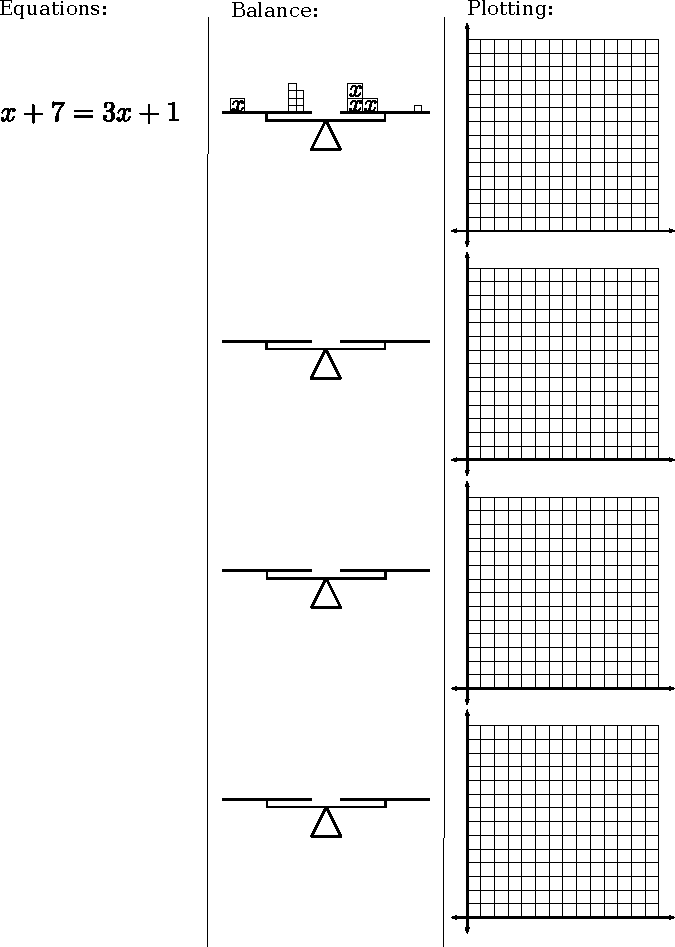
\includegraphics[scale=0.8]{eqBalGraph.pdf}
\end{image}
\end{problem}


\begin{problem}
Critically analyze the three ``different'' methods of solving
equations, noting the advantages and disadvantages of each. 
\end{problem}

\begin{problem}
Can you solve quadratic equations using the methods above?
If so give an example. If not, explain why not.
\end{problem}

\begin{teachingnote}
The key point here is that it is difficult to make ``balances'' work for anything but linear equations.  But the graphical approach always works, as described in the following standard:  

CCSS.A-REI.11.  Explain why the $x$-coordinates of the points where the graphs of the equations $y = f(x)$ and $y = g(x)$ intersect are the solutions of the equation $f(x) = g(x)$; find the solutions approximately, e.g., using technology to graph the functions, make tables of values, or find successive approximations. Include cases where $f(x)$ and/or $g(x)$ are linear, polynomial, rational, absolute value, exponential, and logarithmic functions.*
\end{teachingnote}


\begin{problem}
Can you think of an example when the undoing via algebraic
manipulation would fail?
\end{problem}

\begin{teachingnote}
Here we are looking for something where an inverse function must be
applied, as in $0.6 = \sin(x)$.
\end{teachingnote}


While sometimes we solve equations via a process of algebraic
manipulation, other times we have a formula.


\begin{problem}
Give a formula for solving linear equations of the form $ax + b =0$.
\end{problem}

\end{document}
